\documentclass[10pt, a4paper]{article}
%%%%%%%%%%%%%%%%%%%
% ZA KODO
\usepackage[breakable]{tcolorbox}
    \usepackage{parskip} % Stop auto-indenting (to mimic markdown behaviour)
    
    \usepackage{iftex}
    \ifPDFTeX
    	\usepackage[T1]{fontenc}
    	\usepackage{mathpazo}
    \else
    	\usepackage{fontspec}
    \fi

    % Basic figure setup, for now with no caption control since it's done
    % automatically by Pandoc (which extracts ![](path) syntax from Markdown).
    \usepackage{graphicx}
    % Maintain compatibility with old templates. Remove in nbconvert 6.0
    \let\Oldincludegraphics\includegraphics
    % Ensure that by default, figures have no caption (until we provide a
    % proper Figure object with a Caption API and a way to capture that
    % in the conversion process - todo).
    \usepackage{caption}
    \DeclareCaptionFormat{nocaption}{}
    \captionsetup{format=nocaption,aboveskip=0pt,belowskip=0pt}

    \usepackage[Export]{adjustbox} % Used to constrain images to a maximum size
    \adjustboxset{max size={0.9\linewidth}{0.9\paperheight}}
    \usepackage{float}
    \floatplacement{figure}{H} % forces figures to be placed at the correct location
    \usepackage{xcolor} % Allow colors to be defined
    \usepackage{enumerate} % Needed for markdown enumerations to work
    \usepackage{geometry} % Used to adjust the document margins
    \usepackage{amsmath} % Equations
    \usepackage{amssymb} % Equations
    \usepackage{textcomp} % defines textquotesingle
    % Hack from http://tex.stackexchange.com/a/47451/13684:
    \AtBeginDocument{%
        \def\PYZsq{\textquotesingle}% Upright quotes in Pygmentized code
    }
    \usepackage{upquote} % Upright quotes for verbatim code
    \usepackage{eurosym} % defines \euro
    \usepackage[mathletters]{ucs} % Extended unicode (utf-8) support
    \usepackage{fancyvrb} % verbatim replacement that allows latex
    \usepackage{grffile} % extends the file name processing of package graphics 
                         % to support a larger range
    \makeatletter % fix for grffile with XeLaTeX
    \def\Gread@@xetex#1{%
      \IfFileExists{"\Gin@base".bb}%
      {\Gread@eps{\Gin@base.bb}}%
      {\Gread@@xetex@aux#1}%
    }
    \makeatother

    % The hyperref package gives us a pdf with properly built
    % internal navigation ('pdf bookmarks' for the table of contents,
    % internal cross-reference links, web links for URLs, etc.)
    \usepackage{hyperref}
    % The default LaTeX title has an obnoxious amount of whitespace. By default,
    % titling removes some of it. It also provides customization options.
    \usepackage{titling}
    \usepackage{longtable} % longtable support required by pandoc >1.10
    \usepackage{booktabs}  % table support for pandoc > 1.12.2
    \usepackage[inline]{enumitem} % IRkernel/repr support (it uses the enumerate* environment)
    \usepackage[normalem]{ulem} % ulem is needed to support strikethroughs (\sout)
                                % normalem makes italics be italics, not underlines
    \usepackage{mathrsfs}
    

    
    % Colors for the hyperref package
    \definecolor{urlcolor}{rgb}{0,.145,.698}
    \definecolor{linkcolor}{rgb}{.71,0.21,0.01}
    \definecolor{citecolor}{rgb}{.12,.54,.11}

    % ANSI colors
    \definecolor{ansi-black}{HTML}{3E424D}
    \definecolor{ansi-black-intense}{HTML}{282C36}
    \definecolor{ansi-red}{HTML}{E75C58}
    \definecolor{ansi-red-intense}{HTML}{B22B31}
    \definecolor{ansi-green}{HTML}{00A250}
    \definecolor{ansi-green-intense}{HTML}{007427}
    \definecolor{ansi-yellow}{HTML}{DDB62B}
    \definecolor{ansi-yellow-intense}{HTML}{B27D12}
    \definecolor{ansi-blue}{HTML}{208FFB}
    \definecolor{ansi-blue-intense}{HTML}{0065CA}
    \definecolor{ansi-magenta}{HTML}{D160C4}
    \definecolor{ansi-magenta-intense}{HTML}{A03196}
    \definecolor{ansi-cyan}{HTML}{60C6C8}
    \definecolor{ansi-cyan-intense}{HTML}{258F8F}
    \definecolor{ansi-white}{HTML}{C5C1B4}
    \definecolor{ansi-white-intense}{HTML}{A1A6B2}
    \definecolor{ansi-default-inverse-fg}{HTML}{FFFFFF}
    \definecolor{ansi-default-inverse-bg}{HTML}{000000}

    % commands and environments needed by pandoc snippets
    % extracted from the output of `pandoc -s`
    \providecommand{\tightlist}{%
      \setlength{\itemsep}{0pt}\setlength{\parskip}{0pt}}
    \DefineVerbatimEnvironment{Highlighting}{Verbatim}{commandchars=\\\{\}}
    % Add ',fontsize=\small' for more characters per line
    \newenvironment{Shaded}{}{}
    \newcommand{\KeywordTok}[1]{\textcolor[rgb]{0.00,0.44,0.13}{\textbf{{#1}}}}
    \newcommand{\DataTypeTok}[1]{\textcolor[rgb]{0.56,0.13,0.00}{{#1}}}
    \newcommand{\DecValTok}[1]{\textcolor[rgb]{0.25,0.63,0.44}{{#1}}}
    \newcommand{\BaseNTok}[1]{\textcolor[rgb]{0.25,0.63,0.44}{{#1}}}
    \newcommand{\FloatTok}[1]{\textcolor[rgb]{0.25,0.63,0.44}{{#1}}}
    \newcommand{\CharTok}[1]{\textcolor[rgb]{0.25,0.44,0.63}{{#1}}}
    \newcommand{\StringTok}[1]{\textcolor[rgb]{0.25,0.44,0.63}{{#1}}}
    \newcommand{\CommentTok}[1]{\textcolor[rgb]{0.38,0.63,0.69}{\textit{{#1}}}}
    \newcommand{\OtherTok}[1]{\textcolor[rgb]{0.00,0.44,0.13}{{#1}}}
    \newcommand{\AlertTok}[1]{\textcolor[rgb]{1.00,0.00,0.00}{\textbf{{#1}}}}
    \newcommand{\FunctionTok}[1]{\textcolor[rgb]{0.02,0.16,0.49}{{#1}}}
    \newcommand{\RegionMarkerTok}[1]{{#1}}
    \newcommand{\ErrorTok}[1]{\textcolor[rgb]{1.00,0.00,0.00}{\textbf{{#1}}}}
    \newcommand{\NormalTok}[1]{{#1}}
    
    % Additional commands for more recent versions of Pandoc
    \newcommand{\ConstantTok}[1]{\textcolor[rgb]{0.53,0.00,0.00}{{#1}}}
    \newcommand{\SpecialCharTok}[1]{\textcolor[rgb]{0.25,0.44,0.63}{{#1}}}
    \newcommand{\VerbatimStringTok}[1]{\textcolor[rgb]{0.25,0.44,0.63}{{#1}}}
    \newcommand{\SpecialStringTok}[1]{\textcolor[rgb]{0.73,0.40,0.53}{{#1}}}
    \newcommand{\ImportTok}[1]{{#1}}
    \newcommand{\DocumentationTok}[1]{\textcolor[rgb]{0.73,0.13,0.13}{\textit{{#1}}}}
    \newcommand{\AnnotationTok}[1]{\textcolor[rgb]{0.38,0.63,0.69}{\textbf{\textit{{#1}}}}}
    \newcommand{\CommentVarTok}[1]{\textcolor[rgb]{0.38,0.63,0.69}{\textbf{\textit{{#1}}}}}
    \newcommand{\VariableTok}[1]{\textcolor[rgb]{0.10,0.09,0.49}{{#1}}}
    \newcommand{\ControlFlowTok}[1]{\textcolor[rgb]{0.00,0.44,0.13}{\textbf{{#1}}}}
    \newcommand{\OperatorTok}[1]{\textcolor[rgb]{0.40,0.40,0.40}{{#1}}}
    \newcommand{\BuiltInTok}[1]{{#1}}
    \newcommand{\ExtensionTok}[1]{{#1}}
    \newcommand{\PreprocessorTok}[1]{\textcolor[rgb]{0.74,0.48,0.00}{{#1}}}
    \newcommand{\AttributeTok}[1]{\textcolor[rgb]{0.49,0.56,0.16}{{#1}}}
    \newcommand{\InformationTok}[1]{\textcolor[rgb]{0.38,0.63,0.69}{\textbf{\textit{{#1}}}}}
    \newcommand{\WarningTok}[1]{\textcolor[rgb]{0.38,0.63,0.69}{\textbf{\textit{{#1}}}}}
    
    
    % Define a nice break command that doesn't care if a line doesn't already
    % exist.
    \def\br{\hspace*{\fill} \\* }
    % Math Jax compatibility definitions
    \def\gt{>}
    \def\lt{<}
    \let\Oldtex\TeX
    \let\Oldlatex\LaTeX
    \renewcommand{\TeX}{\textrm{\Oldtex}}
    \renewcommand{\LaTeX}{\textrm{\Oldlatex}}
    % Document parameters
    % Document title
    \title{Lepo zapisana koda za porocilo}
    
    
    
    
    
% Pygments definitions
\makeatletter
\def\PY@reset{\let\PY@it=\relax \let\PY@bf=\relax%
    \let\PY@ul=\relax \let\PY@tc=\relax%
    \let\PY@bc=\relax \let\PY@ff=\relax}
\def\PY@tok#1{\csname PY@tok@#1\endcsname}
\def\PY@toks#1+{\ifx\relax#1\empty\else%
    \PY@tok{#1}\expandafter\PY@toks\fi}
\def\PY@do#1{\PY@bc{\PY@tc{\PY@ul{%
    \PY@it{\PY@bf{\PY@ff{#1}}}}}}}
\def\PY#1#2{\PY@reset\PY@toks#1+\relax+\PY@do{#2}}

\expandafter\def\csname PY@tok@w\endcsname{\def\PY@tc##1{\textcolor[rgb]{0.73,0.73,0.73}{##1}}}
\expandafter\def\csname PY@tok@c\endcsname{\let\PY@it=\textit\def\PY@tc##1{\textcolor[rgb]{0.25,0.50,0.50}{##1}}}
\expandafter\def\csname PY@tok@cp\endcsname{\def\PY@tc##1{\textcolor[rgb]{0.74,0.48,0.00}{##1}}}
\expandafter\def\csname PY@tok@k\endcsname{\let\PY@bf=\textbf\def\PY@tc##1{\textcolor[rgb]{0.00,0.50,0.00}{##1}}}
\expandafter\def\csname PY@tok@kp\endcsname{\def\PY@tc##1{\textcolor[rgb]{0.00,0.50,0.00}{##1}}}
\expandafter\def\csname PY@tok@kt\endcsname{\def\PY@tc##1{\textcolor[rgb]{0.69,0.00,0.25}{##1}}}
\expandafter\def\csname PY@tok@o\endcsname{\def\PY@tc##1{\textcolor[rgb]{0.40,0.40,0.40}{##1}}}
\expandafter\def\csname PY@tok@ow\endcsname{\let\PY@bf=\textbf\def\PY@tc##1{\textcolor[rgb]{0.67,0.13,1.00}{##1}}}
\expandafter\def\csname PY@tok@nb\endcsname{\def\PY@tc##1{\textcolor[rgb]{0.00,0.50,0.00}{##1}}}
\expandafter\def\csname PY@tok@nf\endcsname{\def\PY@tc##1{\textcolor[rgb]{0.00,0.00,1.00}{##1}}}
\expandafter\def\csname PY@tok@nc\endcsname{\let\PY@bf=\textbf\def\PY@tc##1{\textcolor[rgb]{0.00,0.00,1.00}{##1}}}
\expandafter\def\csname PY@tok@nn\endcsname{\let\PY@bf=\textbf\def\PY@tc##1{\textcolor[rgb]{0.00,0.00,1.00}{##1}}}
\expandafter\def\csname PY@tok@ne\endcsname{\let\PY@bf=\textbf\def\PY@tc##1{\textcolor[rgb]{0.82,0.25,0.23}{##1}}}
\expandafter\def\csname PY@tok@nv\endcsname{\def\PY@tc##1{\textcolor[rgb]{0.10,0.09,0.49}{##1}}}
\expandafter\def\csname PY@tok@no\endcsname{\def\PY@tc##1{\textcolor[rgb]{0.53,0.00,0.00}{##1}}}
\expandafter\def\csname PY@tok@nl\endcsname{\def\PY@tc##1{\textcolor[rgb]{0.63,0.63,0.00}{##1}}}
\expandafter\def\csname PY@tok@ni\endcsname{\let\PY@bf=\textbf\def\PY@tc##1{\textcolor[rgb]{0.60,0.60,0.60}{##1}}}
\expandafter\def\csname PY@tok@na\endcsname{\def\PY@tc##1{\textcolor[rgb]{0.49,0.56,0.16}{##1}}}
\expandafter\def\csname PY@tok@nt\endcsname{\let\PY@bf=\textbf\def\PY@tc##1{\textcolor[rgb]{0.00,0.50,0.00}{##1}}}
\expandafter\def\csname PY@tok@nd\endcsname{\def\PY@tc##1{\textcolor[rgb]{0.67,0.13,1.00}{##1}}}
\expandafter\def\csname PY@tok@s\endcsname{\def\PY@tc##1{\textcolor[rgb]{0.73,0.13,0.13}{##1}}}
\expandafter\def\csname PY@tok@sd\endcsname{\let\PY@it=\textit\def\PY@tc##1{\textcolor[rgb]{0.73,0.13,0.13}{##1}}}
\expandafter\def\csname PY@tok@si\endcsname{\let\PY@bf=\textbf\def\PY@tc##1{\textcolor[rgb]{0.73,0.40,0.53}{##1}}}
\expandafter\def\csname PY@tok@se\endcsname{\let\PY@bf=\textbf\def\PY@tc##1{\textcolor[rgb]{0.73,0.40,0.13}{##1}}}
\expandafter\def\csname PY@tok@sr\endcsname{\def\PY@tc##1{\textcolor[rgb]{0.73,0.40,0.53}{##1}}}
\expandafter\def\csname PY@tok@ss\endcsname{\def\PY@tc##1{\textcolor[rgb]{0.10,0.09,0.49}{##1}}}
\expandafter\def\csname PY@tok@sx\endcsname{\def\PY@tc##1{\textcolor[rgb]{0.00,0.50,0.00}{##1}}}
\expandafter\def\csname PY@tok@m\endcsname{\def\PY@tc##1{\textcolor[rgb]{0.40,0.40,0.40}{##1}}}
\expandafter\def\csname PY@tok@gh\endcsname{\let\PY@bf=\textbf\def\PY@tc##1{\textcolor[rgb]{0.00,0.00,0.50}{##1}}}
\expandafter\def\csname PY@tok@gu\endcsname{\let\PY@bf=\textbf\def\PY@tc##1{\textcolor[rgb]{0.50,0.00,0.50}{##1}}}
\expandafter\def\csname PY@tok@gd\endcsname{\def\PY@tc##1{\textcolor[rgb]{0.63,0.00,0.00}{##1}}}
\expandafter\def\csname PY@tok@gi\endcsname{\def\PY@tc##1{\textcolor[rgb]{0.00,0.63,0.00}{##1}}}
\expandafter\def\csname PY@tok@gr\endcsname{\def\PY@tc##1{\textcolor[rgb]{1.00,0.00,0.00}{##1}}}
\expandafter\def\csname PY@tok@ge\endcsname{\let\PY@it=\textit}
\expandafter\def\csname PY@tok@gs\endcsname{\let\PY@bf=\textbf}
\expandafter\def\csname PY@tok@gp\endcsname{\let\PY@bf=\textbf\def\PY@tc##1{\textcolor[rgb]{0.00,0.00,0.50}{##1}}}
\expandafter\def\csname PY@tok@go\endcsname{\def\PY@tc##1{\textcolor[rgb]{0.53,0.53,0.53}{##1}}}
\expandafter\def\csname PY@tok@gt\endcsname{\def\PY@tc##1{\textcolor[rgb]{0.00,0.27,0.87}{##1}}}
\expandafter\def\csname PY@tok@err\endcsname{\def\PY@bc##1{\setlength{\fboxsep}{0pt}\fcolorbox[rgb]{1.00,0.00,0.00}{1,1,1}{\strut ##1}}}
\expandafter\def\csname PY@tok@kc\endcsname{\let\PY@bf=\textbf\def\PY@tc##1{\textcolor[rgb]{0.00,0.50,0.00}{##1}}}
\expandafter\def\csname PY@tok@kd\endcsname{\let\PY@bf=\textbf\def\PY@tc##1{\textcolor[rgb]{0.00,0.50,0.00}{##1}}}
\expandafter\def\csname PY@tok@kn\endcsname{\let\PY@bf=\textbf\def\PY@tc##1{\textcolor[rgb]{0.00,0.50,0.00}{##1}}}
\expandafter\def\csname PY@tok@kr\endcsname{\let\PY@bf=\textbf\def\PY@tc##1{\textcolor[rgb]{0.00,0.50,0.00}{##1}}}
\expandafter\def\csname PY@tok@bp\endcsname{\def\PY@tc##1{\textcolor[rgb]{0.00,0.50,0.00}{##1}}}
\expandafter\def\csname PY@tok@fm\endcsname{\def\PY@tc##1{\textcolor[rgb]{0.00,0.00,1.00}{##1}}}
\expandafter\def\csname PY@tok@vc\endcsname{\def\PY@tc##1{\textcolor[rgb]{0.10,0.09,0.49}{##1}}}
\expandafter\def\csname PY@tok@vg\endcsname{\def\PY@tc##1{\textcolor[rgb]{0.10,0.09,0.49}{##1}}}
\expandafter\def\csname PY@tok@vi\endcsname{\def\PY@tc##1{\textcolor[rgb]{0.10,0.09,0.49}{##1}}}
\expandafter\def\csname PY@tok@vm\endcsname{\def\PY@tc##1{\textcolor[rgb]{0.10,0.09,0.49}{##1}}}
\expandafter\def\csname PY@tok@sa\endcsname{\def\PY@tc##1{\textcolor[rgb]{0.73,0.13,0.13}{##1}}}
\expandafter\def\csname PY@tok@sb\endcsname{\def\PY@tc##1{\textcolor[rgb]{0.73,0.13,0.13}{##1}}}
\expandafter\def\csname PY@tok@sc\endcsname{\def\PY@tc##1{\textcolor[rgb]{0.73,0.13,0.13}{##1}}}
\expandafter\def\csname PY@tok@dl\endcsname{\def\PY@tc##1{\textcolor[rgb]{0.73,0.13,0.13}{##1}}}
\expandafter\def\csname PY@tok@s2\endcsname{\def\PY@tc##1{\textcolor[rgb]{0.73,0.13,0.13}{##1}}}
\expandafter\def\csname PY@tok@sh\endcsname{\def\PY@tc##1{\textcolor[rgb]{0.73,0.13,0.13}{##1}}}
\expandafter\def\csname PY@tok@s1\endcsname{\def\PY@tc##1{\textcolor[rgb]{0.73,0.13,0.13}{##1}}}
\expandafter\def\csname PY@tok@mb\endcsname{\def\PY@tc##1{\textcolor[rgb]{0.40,0.40,0.40}{##1}}}
\expandafter\def\csname PY@tok@mf\endcsname{\def\PY@tc##1{\textcolor[rgb]{0.40,0.40,0.40}{##1}}}
\expandafter\def\csname PY@tok@mh\endcsname{\def\PY@tc##1{\textcolor[rgb]{0.40,0.40,0.40}{##1}}}
\expandafter\def\csname PY@tok@mi\endcsname{\def\PY@tc##1{\textcolor[rgb]{0.40,0.40,0.40}{##1}}}
\expandafter\def\csname PY@tok@il\endcsname{\def\PY@tc##1{\textcolor[rgb]{0.40,0.40,0.40}{##1}}}
\expandafter\def\csname PY@tok@mo\endcsname{\def\PY@tc##1{\textcolor[rgb]{0.40,0.40,0.40}{##1}}}
\expandafter\def\csname PY@tok@ch\endcsname{\let\PY@it=\textit\def\PY@tc##1{\textcolor[rgb]{0.25,0.50,0.50}{##1}}}
\expandafter\def\csname PY@tok@cm\endcsname{\let\PY@it=\textit\def\PY@tc##1{\textcolor[rgb]{0.25,0.50,0.50}{##1}}}
\expandafter\def\csname PY@tok@cpf\endcsname{\let\PY@it=\textit\def\PY@tc##1{\textcolor[rgb]{0.25,0.50,0.50}{##1}}}
\expandafter\def\csname PY@tok@c1\endcsname{\let\PY@it=\textit\def\PY@tc##1{\textcolor[rgb]{0.25,0.50,0.50}{##1}}}
\expandafter\def\csname PY@tok@cs\endcsname{\let\PY@it=\textit\def\PY@tc##1{\textcolor[rgb]{0.25,0.50,0.50}{##1}}}

\def\PYZbs{\char`\\}
\def\PYZus{\char`\_}
\def\PYZob{\char`\{}
\def\PYZcb{\char`\}}
\def\PYZca{\char`\^}
\def\PYZam{\char`\&}
\def\PYZlt{\char`\<}
\def\PYZgt{\char`\>}
\def\PYZsh{\char`\#}
\def\PYZpc{\char`\%}
\def\PYZdl{\char`\$}
\def\PYZhy{\char`\-}
\def\PYZsq{\char`\'}
\def\PYZdq{\char`\"}
\def\PYZti{\char`\~}
% for compatibility with earlier versions
\def\PYZat{@}
\def\PYZlb{[}
\def\PYZrb{]}
\makeatother


    % For linebreaks inside Verbatim environment from package fancyvrb. 
    \makeatletter
        \newbox\Wrappedcontinuationbox 
        \newbox\Wrappedvisiblespacebox 
        \newcommand*\Wrappedvisiblespace {\textcolor{red}{\textvisiblespace}} 
        \newcommand*\Wrappedcontinuationsymbol {\textcolor{red}{\llap{\tiny$\m@th\hookrightarrow$}}} 
        \newcommand*\Wrappedcontinuationindent {3ex } 
        \newcommand*\Wrappedafterbreak {\kern\Wrappedcontinuationindent\copy\Wrappedcontinuationbox} 
        % Take advantage of the already applied Pygments mark-up to insert 
        % potential linebreaks for TeX processing. 
        %        {, <, #, %, $, ' and ": go to next line. 
        %        _, }, ^, &, >, - and ~: stay at end of broken line. 
        % Use of \textquotesingle for straight quote. 
        \newcommand*\Wrappedbreaksatspecials {% 
            \def\PYGZus{\discretionary{\char`\_}{\Wrappedafterbreak}{\char`\_}}% 
            \def\PYGZob{\discretionary{}{\Wrappedafterbreak\char`\{}{\char`\{}}% 
            \def\PYGZcb{\discretionary{\char`\}}{\Wrappedafterbreak}{\char`\}}}% 
            \def\PYGZca{\discretionary{\char`\^}{\Wrappedafterbreak}{\char`\^}}% 
            \def\PYGZam{\discretionary{\char`\&}{\Wrappedafterbreak}{\char`\&}}% 
            \def\PYGZlt{\discretionary{}{\Wrappedafterbreak\char`\<}{\char`\<}}% 
            \def\PYGZgt{\discretionary{\char`\>}{\Wrappedafterbreak}{\char`\>}}% 
            \def\PYGZsh{\discretionary{}{\Wrappedafterbreak\char`\#}{\char`\#}}% 
            \def\PYGZpc{\discretionary{}{\Wrappedafterbreak\char`\%}{\char`\%}}% 
            \def\PYGZdl{\discretionary{}{\Wrappedafterbreak\char`\$}{\char`\$}}% 
            \def\PYGZhy{\discretionary{\char`\-}{\Wrappedafterbreak}{\char`\-}}% 
            \def\PYGZsq{\discretionary{}{\Wrappedafterbreak\textquotesingle}{\textquotesingle}}% 
            \def\PYGZdq{\discretionary{}{\Wrappedafterbreak\char`\"}{\char`\"}}% 
            \def\PYGZti{\discretionary{\char`\~}{\Wrappedafterbreak}{\char`\~}}% 
        } 
        % Some characters . , ; ? ! / are not pygmentized. 
        % This macro makes them "active" and they will insert potential linebreaks 
        \newcommand*\Wrappedbreaksatpunct {% 
            \lccode`\~`\.\lowercase{\def~}{\discretionary{\hbox{\char`\.}}{\Wrappedafterbreak}{\hbox{\char`\.}}}% 
            \lccode`\~`\,\lowercase{\def~}{\discretionary{\hbox{\char`\,}}{\Wrappedafterbreak}{\hbox{\char`\,}}}% 
            \lccode`\~`\;\lowercase{\def~}{\discretionary{\hbox{\char`\;}}{\Wrappedafterbreak}{\hbox{\char`\;}}}% 
            \lccode`\~`\:\lowercase{\def~}{\discretionary{\hbox{\char`\:}}{\Wrappedafterbreak}{\hbox{\char`\:}}}% 
            \lccode`\~`\?\lowercase{\def~}{\discretionary{\hbox{\char`\?}}{\Wrappedafterbreak}{\hbox{\char`\?}}}% 
            \lccode`\~`\!\lowercase{\def~}{\discretionary{\hbox{\char`\!}}{\Wrappedafterbreak}{\hbox{\char`\!}}}% 
            \lccode`\~`\/\lowercase{\def~}{\discretionary{\hbox{\char`\/}}{\Wrappedafterbreak}{\hbox{\char`\/}}}% 
            \catcode`\.\active
            \catcode`\,\active 
            \catcode`\;\active
            \catcode`\:\active
            \catcode`\?\active
            \catcode`\!\active
            \catcode`\/\active 
            \lccode`\~`\~ 	
        }
    \makeatother

    \let\OriginalVerbatim=\Verbatim
    \makeatletter
    \renewcommand{\Verbatim}[1][1]{%
        %\parskip\z@skip
        \sbox\Wrappedcontinuationbox {\Wrappedcontinuationsymbol}%
        \sbox\Wrappedvisiblespacebox {\FV@SetupFont\Wrappedvisiblespace}%
        \def\FancyVerbFormatLine ##1{\hsize\linewidth
            \vtop{\raggedright\hyphenpenalty\z@\exhyphenpenalty\z@
                \doublehyphendemerits\z@\finalhyphendemerits\z@
                \strut ##1\strut}%
        }%
        % If the linebreak is at a space, the latter will be displayed as visible
        % space at end of first line, and a continuation symbol starts next line.
        % Stretch/shrink are however usually zero for typewriter font.
        \def\FV@Space {%
            \nobreak\hskip\z@ plus\fontdimen3\font minus\fontdimen4\font
            \discretionary{\copy\Wrappedvisiblespacebox}{\Wrappedafterbreak}
            {\kern\fontdimen2\font}%
        }%
        
        % Allow breaks at special characters using \PYG... macros.
        \Wrappedbreaksatspecials
        % Breaks at punctuation characters . , ; ? ! and / need catcode=\active 	
        \OriginalVerbatim[#1,codes*=\Wrappedbreaksatpunct]%
    }
    \makeatother

    % Exact colors from NB
    \definecolor{incolor}{HTML}{303F9F}
    \definecolor{outcolor}{HTML}{D84315}
    \definecolor{cellborder}{HTML}{CFCFCF}
    \definecolor{cellbackground}{HTML}{F7F7F7}
    
    % prompt
    \makeatletter
    \newcommand{\boxspacing}{\kern\kvtcb@left@rule\kern\kvtcb@boxsep}
    \makeatother
    \newcommand{\prompt}[4]{
        \ttfamily\llap{{\color{#2}[#3]:\hspace{3pt}#4}}\vspace{-\baselineskip}
    }
    

    
    % Prevent overflowing lines due to hard-to-break entities
    \sloppy 
    % Setup hyperref package
    \hypersetup{
      breaklinks=true,  % so long urls are correctly broken across lines
      colorlinks=true,
      urlcolor=urlcolor,
      linkcolor=linkcolor,
      citecolor=citecolor,
      }
    % Slightly bigger margins than the latex defaults
    
    \geometry{verbose,tmargin=1in,bmargin=1in,lmargin=1in,rmargin=1in}

%%%%%%%%%%%%%%%%%%%
\usepackage[slovene]{babel}
\usepackage[utf8]{inputenc} %za šumnike
\usepackage{lmodern}
\usepackage[T1]{fontenc}
\usepackage{eurosym}

%slike:
\usepackage{graphicx}
\graphicspath{ {./slike/} }

\begin{document}

\begin{center}
\Huge \textbf{Naslov Skupina 19: Graffiti conjecture 232} \\
\medskip
\Large Urban Merhar, Martin Kokošinek\\
\end{center}

\section{Navodilo}
Računalniško generirana domneva trdi: Če je $G$ enostaven povezan graf, potem
\begin{center}
 $2\gamma_{t}(G) \geq rad(G) + ecc(B)$.
\end{center}
 
Preveri domnevo na različne načine za male in velike grafe. Z uporabo populacijske metahevristike, preveri domnevo v upanju, da jo ovržeš.

\medskip
Nekaj pripomb:

\begin{enumerate}
\item $ecc(v)$ je $ekscentričnost$ od vozlišča $v$. Ekscentričnost od $v$ je razdalja do najbolj oddaljenega vozlišča od vozlišča $v$, i.e., $ max\{d(v,u): u$ je vozlišče na grafu $\}$.
\item $rad(G)$ je $radij$ grafa, t.j., minimum vseh ekscentričnosti vozlišč grafa $G$.
\item $B$ je $obrobje$ grafa $G$, t.j., množica vozlišč z maksimalno ekscentričnostjo.
\item $ecc(S)$ je $ekscentričnost$ množice vozlišč $S$. Definirana je kot: Naj bo $S$ podmnožica množice vozlišč $V$. Razdalja med vozliščem $v$ in množico $S$, definirajmo kot razdaljo od $v$ do najbližjega volišča v $S$. $ecc(S)$ je maksimum razadalj od vozlišča v $V\backslash S$ do množice $S$.
\end{enumerate}


\section{Kratek opis}
$Computer\ generated\ conjectures$ so računalniško ustvarjene domneve. $Graffiti$ je računalniški program, ki generira te matematične domneve oziroma odprte probleme. Računalniši program $Graffiti$ je ustvaril $Siemion\ Fajtlowicz$.\\

V najinem projektu pri predmetu Finančni praktikum si bova ogledala $Graffiti$ $conjecture$ $232$, ki jo bova testirala za majhne in velike grafe v upanju, da najdeva protiprimer. Ideja je, da enačbo zapiševa v programskem jeziku $Sage$ in generirava naključne grafe. Na vsakem od teh grafov pa predpostavko testirava.\\


Že vgrajene funkcije, ki jih bova uporabila v programu:
\begin{enumerate}
	\item $dominating\_ set(total=True, value\_ only=True)$ vrne najmanjšo dominirajočo množico na grafu $G$.
	\item $radius()$ vrne radij grafa $G$.
	\item $eccentricity()$ vrne ekscentričnost vozlišča $v$.
	\item $periphery()$ vrne množico vozlišč iz obrobja grafa $G$.
\end{enumerate}

\subsection{Razlaga pojmov}
\begin{itemize}
\item Dominirajoča Množica $D$: $D$ je množica, kjer je vsako vozlišče iz $G \backslash D$ sosed nekega vozlišča iz $D$.
\item Totalno Dominirajoča množica (TDM): Dominirajoči množici $D$ dodamo pogoj, da so tudi vozlišča dominirajoče množice 
$D$ sosedi vozlišč iz $D$.
\item Totalno Dominirajoče Število (TDŠ): Moč totalno dominirajoče množice grafa $G$.
\item $\gamma_{t}(G)$ je TDŠ grafa $G$.
\end{itemize}

\subsubsection{Populacijska metahevristika}
\textbf{Hevristika} (iz Grščine: 'najdem, odkrijem'): V računalništvu in matematični optimizaciji je visoko-nivojski način reševanja problemov, ko so klasični postopki prepočasni oziroma, ko klasične metode ne vrnejo točnih rezultatov. V zameno za polnost, optimalnost, natančnost, raje pridobimo na časovni zahtevnosti. \\
\textbf{Meta-hevristika} (meta iz Grščine: 'za, onstran') oziroma v prevodu Izčrpna-hevristika: Metahevristika vzame množico rešitev, ki je prevelika za analizo in s pomočjo določenih predpostavk glede optimizacije vrne zadovoljivo rešitev. Ta ni nujno globalno optimalna. \\
\textbf{Populacijska metahevristika}: Ohranjamo večje število kandidatov za rešitev in jih izboljšujemo s pomočjo populacijsih karakteristik. Primer je particle swarm optimization (PSO).

\section{Plan dela}
Zapisati učinkovit algoritem, ki bo za vsak generiran graf preverila lastnosti grafa in posledično domnevo. Za grafe, kjer  domneva ne bi držala pa nam izpiše graf in vrne vrednosti lastnosti, ki so potrebovane v domnevi.

\section{Potek dela}

Za preverjanje dane domneve sva napisala program, ki jo testira. Samo domnevo pa sva nekoliko obrnila na način, da lahko učinkovito gledava tudi njeno razliko. To sva storila z namenom da opazujeva kateri grafi so bližje temu, da bi bili lahko protiprimer domneve. Kot je vidno v spodnjem programu sva tako na grafih preverjala $2\gamma_{t}(G) - rad(G) - ecc(B) \geq 0$. Na ta način sva s pomočjo razlike $2\gamma_{t}(G) - rad(G) - ecc(B)$ ocenjevala kako blizu pride nek graf k temu, da bi bil protiprimer.

Funkcija z imenom $predpostavka()$ sprejme dan graf $G$ in na njem testira domnevo ter vrne razliko $2\gamma_{t}(G) - rad(G) - ecc(B)$, če predpostavka velja, sicer pa pove, da predpostavka ne velja. 

V spodnji kodi je naveden še primer in potek izračuna vrednosti domneve ter tudi način generiranja velikih in malih grafov.

%%%%%KODA%%%%%%%%%%%%%%%%%%%%%%%%%%%%%%%%%%%%%%%%%%%%%
    \begin{tcolorbox}[breakable, size=fbox, boxrule=1pt, pad at break*=1mm,colback=cellbackground, colframe=cellborder]
\prompt{In}{incolor}{1}{\boxspacing}
\begin{Verbatim}[commandchars=\\\{\}]
\PY{c+c1}{\PYZsh{} Projektna naloga pri predmetu Financni praktikum}

\PY{c+c1}{\PYZsh{} Naloga 19: Graffiti conjecture 232}

\PY{k}{def} \PY{n+nf}{predpostavka}\PY{p}{(}\PY{n}{G}\PY{p}{)}\PY{p}{:}
    \PY{l+s+sd}{\PYZsq{}\PYZsq{}\PYZsq{}Funkcija, ki testira predpostavko Graffiti conjecture 232.\PYZsq{}\PYZsq{}\PYZsq{}}
    \PY{k}{if} \PY{n}{G}\PY{o}{.}\PY{n}{is\PYZus{}connected}\PY{p}{(}\PY{p}{)} \PY{o}{==} \PY{n+nb+bp}{False}\PY{p}{:}
        \PY{k}{return}\PY{p}{(}\PY{l+s+s1}{\PYZsq{}}\PY{l+s+s1}{Graf ni povezan!}\PY{l+s+s1}{\PYZsq{}}\PY{p}{)}
    \PY{n}{B} \PY{o}{=} \PY{n+nb}{set}\PY{p}{(}\PY{n}{G}\PY{o}{.}\PY{n}{periphery}\PY{p}{(}\PY{p}{)}\PY{p}{)}
    \PY{n}{d} \PY{o}{=} \PY{n}{G}\PY{o}{.}\PY{n}{distance\PYZus{}all\PYZus{}pairs}\PY{p}{(}\PY{p}{)}
    \PY{n}{razdalja} \PY{o}{=} \PY{p}{[}\PY{p}{]}
    \PY{k}{for} \PY{n}{v} \PY{o+ow}{in} \PY{n}{G}\PY{p}{:}
        \PY{k}{if} \PY{n}{v} \PY{o+ow}{not} \PY{o+ow}{in} \PY{n}{B}\PY{p}{:}
            \PY{n}{sezv} \PY{o}{=} \PY{p}{[}\PY{p}{]}
            \PY{k}{for} \PY{n}{u} \PY{o+ow}{in} \PY{n}{B}\PY{p}{:}
                \PY{n}{sezv}\PY{o}{.}\PY{n}{append}\PY{p}{(}\PY{n}{d}\PY{p}{[}\PY{n}{v}\PY{p}{]}\PY{p}{[}\PY{n}{u}\PY{p}{]}\PY{p}{)}
            \PY{n}{razdalja}\PY{o}{.}\PY{n}{append}\PY{p}{(}\PY{n+nb}{min}\PY{p}{(}\PY{n}{sezv}\PY{p}{)}\PY{p}{)}
    \PY{n}{razlika} \PY{o}{=} \PY{l+m+mi}{2} \PY{o}{*} \PY{n}{G}\PY{o}{.}\PY{n}{dominating\PYZus{}set}\PY{p}{(}\PY{n}{total}\PY{o}{=}\PY{n+nb+bp}{True}\PY{p}{,} \PY{n}{value\PYZus{}only}\PY{o}{=}\PY{n+nb+bp}{True}\PY{p}{)} \PY{o}{\PYZhy{}} \PY{n}{G}\PY{o}{.}\PY{n}{radius}\PY{p}{(}\PY{p}{)} \PY{o}{\PYZhy{}} \PY{p}{(}\PY{n+nb}{max}\PY{p}{(}\PY{n}{razdalja}\PY{p}{)} \PY{k}{if} \PY{n}{razdalja} \PY{k}{else} \PY{l+m+mi}{0}\PY{p}{)}
    \PY{k}{if} \PY{n}{razlika} \PY{o}{\PYZgt{}}\PY{o}{=} \PY{l+m+mi}{0}\PY{p}{:}
        \PY{k}{print}\PY{p}{(}\PY{l+s+s1}{\PYZsq{}}\PY{l+s+s1}{Razlika med levo in desno stranjo predpostavke je:}\PY{l+s+s1}{\PYZsq{}}\PY{p}{)}
        \PY{k}{print}\PY{p}{(}\PY{n}{razlika}\PY{p}{)}
        \PY{k}{return}\PY{p}{(}\PY{l+s+s1}{\PYZsq{}}\PY{l+s+s1}{Predpostavka velja!}\PY{l+s+s1}{\PYZsq{}}\PY{p}{)}
    \PY{k}{else}\PY{p}{:}
        \PY{k}{return}\PY{p}{(}\PY{l+s+s1}{\PYZsq{}}\PY{l+s+s1}{Predpostavka NE velja!}\PY{l+s+s1}{\PYZsq{}}\PY{p}{)}
\end{Verbatim}
\end{tcolorbox}

    \begin{tcolorbox}[breakable, size=fbox, boxrule=1pt, pad at break*=1mm,colback=cellbackground, colframe=cellborder]
\prompt{In}{incolor}{2}{\boxspacing}
\begin{Verbatim}[commandchars=\\\{\}]
\PY{c+c1}{\PYZsh{} VELIKE GRAFE GENERIRAMO Z:}
\PY{c+c1}{\PYZsh{} graphs.RandomGNP(n, p) generira nakljucni preprost graf kjer je n stevilo vozlisc in p verjetnost povezave med dvema vozliscema}
\PY{n}{G} \PY{o}{=} \PY{n}{graphs}\PY{o}{.}\PY{n}{RandomGNP}\PY{p}{(}\PY{l+m+mi}{5}\PY{p}{,} \PY{l+m+mf}{0.4}\PY{p}{)}
\end{Verbatim}
\end{tcolorbox}

    \begin{tcolorbox}[breakable, size=fbox, boxrule=1pt, pad at break*=1mm,colback=cellbackground, colframe=cellborder]
\prompt{In}{incolor}{3}{\boxspacing}
\begin{Verbatim}[commandchars=\\\{\}]
\PY{n}{G}\PY{o}{.}\PY{n}{show}\PY{p}{(}\PY{p}{)}
\end{Verbatim}
\end{tcolorbox}
 
            
%out slika grafa
\begin{tcolorbox}[breakable, size=fbox, boxrule=.5pt, pad at break*=1mm, opacityfill=0]
\prompt{Out}{outcolor}{3}{\boxspacing}
\begin{Verbatim}[commandchars=\\\{\}]

\end{Verbatim}
\end{tcolorbox}
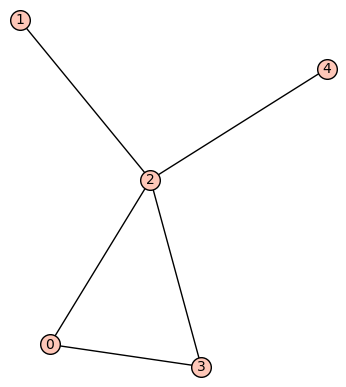
\includegraphics{Lepo zapisana koda za porocilo_2_0.png}
%
 \begin{tcolorbox}[breakable, size=fbox, boxrule=1pt, pad at break*=1mm,colback=cellbackground, colframe=cellborder]
\prompt{In}{incolor}{4}{\boxspacing}
\begin{Verbatim}[commandchars=\\\{\}]
\PY{c+c1}{\PYZsh{} Spodaj so loceno izracunane vse vrednosti v predpostavki}
\end{Verbatim}
\end{tcolorbox}

    \begin{tcolorbox}[breakable, size=fbox, boxrule=1pt, pad at break*=1mm,colback=cellbackground, colframe=cellborder]
\prompt{In}{incolor}{5}{\boxspacing}
\begin{Verbatim}[commandchars=\\\{\}]
\PY{c+c1}{\PYZsh{} total=True da bo total dominating set}
\PY{c+c1}{\PYZsh{} value\PYZus{}only=True \PYZhy{}\PYZgt{} ker nas zanima samo vrednost in ne seznam vozlisc}
\PY{n}{G}\PY{o}{.}\PY{n}{dominating\PYZus{}set}\PY{p}{(}\PY{n}{total}\PY{o}{=}\PY{n+nb+bp}{True}\PY{p}{,} \PY{n}{value\PYZus{}only}\PY{o}{=}\PY{n+nb+bp}{True}\PY{p}{)}
\end{Verbatim}
\end{tcolorbox}

            \begin{tcolorbox}[breakable, size=fbox, boxrule=.5pt, pad at break*=1mm, opacityfill=0]
\prompt{Out}{outcolor}{5}{\boxspacing}
\begin{Verbatim}[commandchars=\\\{\}]
2
\end{Verbatim}
\end{tcolorbox}
        
    \begin{tcolorbox}[breakable, size=fbox, boxrule=1pt, pad at break*=1mm,colback=cellbackground, colframe=cellborder]
\prompt{In}{incolor}{6}{\boxspacing}
\begin{Verbatim}[commandchars=\\\{\}]
\PY{c+c1}{\PYZsh{} radij grafa}
\PY{n}{G}\PY{o}{.}\PY{n}{radius}\PY{p}{(}\PY{p}{)}
\end{Verbatim}
\end{tcolorbox}

            \begin{tcolorbox}[breakable, size=fbox, boxrule=.5pt, pad at break*=1mm, opacityfill=0]
\prompt{Out}{outcolor}{6}{\boxspacing}
\begin{Verbatim}[commandchars=\\\{\}]
2
\end{Verbatim}
\end{tcolorbox}
        
    \begin{tcolorbox}[breakable, size=fbox, boxrule=1pt, pad at break*=1mm,colback=cellbackground, colframe=cellborder]
\prompt{In}{incolor}{7}{\boxspacing}
\begin{Verbatim}[commandchars=\\\{\}]
\PY{c+c1}{\PYZsh{} B je obrobje grafa}
\PY{n}{B} \PY{o}{=} \PY{n+nb}{set}\PY{p}{(}\PY{n}{G}\PY{o}{.}\PY{n}{periphery}\PY{p}{(}\PY{p}{)}\PY{p}{)}
\PY{n}{d} \PY{o}{=} \PY{n}{G}\PY{o}{.}\PY{n}{distance\PYZus{}all\PYZus{}pairs}\PY{p}{(}\PY{p}{)}
\PY{n}{razdalja} \PY{o}{=} \PY{p}{[}\PY{p}{]}
\PY{k}{for} \PY{n}{v} \PY{o+ow}{in} \PY{n}{G}\PY{p}{:}
    \PY{k}{if} \PY{n}{v} \PY{o+ow}{not} \PY{o+ow}{in} \PY{n}{B}\PY{p}{:}
        \PY{n}{sezv} \PY{o}{=} \PY{p}{[}\PY{p}{]}
        \PY{k}{for} \PY{n}{u} \PY{o+ow}{in} \PY{n}{B}\PY{p}{:}
            \PY{n}{sezv}\PY{o}{.}\PY{n}{append}\PY{p}{(}\PY{n}{d}\PY{p}{[}\PY{n}{v}\PY{p}{]}\PY{p}{[}\PY{n}{u}\PY{p}{]}\PY{p}{)}
        \PY{n}{razdalja}\PY{o}{.}\PY{n}{append}\PY{p}{(}\PY{n+nb}{min}\PY{p}{(}\PY{n}{sezv}\PY{p}{)}\PY{p}{)}
\PY{c+c1}{\PYZsh{} razdalja je ekscentricnost obrobja grafa B}
\PY{p}{(}\PY{n+nb}{max}\PY{p}{(}\PY{n}{razdalja}\PY{p}{)} \PY{k}{if} \PY{n}{razdalja} \PY{k}{else} \PY{l+m+mi}{0}\PY{p}{)}
\end{Verbatim}
\end{tcolorbox}

            \begin{tcolorbox}[breakable, size=fbox, boxrule=.5pt, pad at break*=1mm, opacityfill=0]
\prompt{Out}{outcolor}{7}{\boxspacing}
\begin{Verbatim}[commandchars=\\\{\}]
1
\end{Verbatim}
\end{tcolorbox}
        
    \begin{tcolorbox}[breakable, size=fbox, boxrule=1pt, pad at break*=1mm,colback=cellbackground, colframe=cellborder]
\prompt{In}{incolor}{8}{\boxspacing}
\begin{Verbatim}[commandchars=\\\{\}]
\PY{c+c1}{\PYZsh{} Preizkusimo funkcijo na zgornjem grafu:}
\PY{n}{predpostavka}\PY{p}{(}\PY{n}{G}\PY{p}{)}
\end{Verbatim}
\end{tcolorbox}

    \begin{Verbatim}[commandchars=\\\{\}]
Razlika med levo in desno stranjo predpostavke je:
1
    \end{Verbatim}

            \begin{tcolorbox}[breakable, size=fbox, boxrule=.5pt, pad at break*=1mm, opacityfill=0]
\prompt{Out}{outcolor}{8}{\boxspacing}
\begin{Verbatim}[commandchars=\\\{\}]
'Predpostavka velja!'
\end{Verbatim}
\end{tcolorbox}
        
    \begin{tcolorbox}[breakable, size=fbox, boxrule=1pt, pad at break*=1mm,colback=cellbackground, colframe=cellborder]
\prompt{In}{incolor}{9}{\boxspacing}
\begin{Verbatim}[commandchars=\\\{\}]
\PY{c+c1}{\PYZsh{} GENERIRANJE MAJHNIH GRAFOV}
\PY{c+c1}{\PYZsh{} ker grafe generiras z nauty\PYZus{}geng so vsi preprosti (tako pise v dokumentaciji)}
\PY{n}{seznam} \PY{o}{=} \PY{p}{[}\PY{n}{G} \PY{k}{for} \PY{n}{G} \PY{o+ow}{in} \PY{n}{graphs}\PY{o}{.}\PY{n}{nauty\PYZus{}geng}\PY{p}{(}\PY{l+s+s1}{\PYZsq{}}\PY{l+s+s1}{3 \PYZhy{}c}\PY{l+s+s1}{\PYZsq{}}\PY{p}{)}\PY{p}{]} \PY{c+c1}{\PYZsh{} povezani grafi na \PYZdq{}n\PYZdq{} vozliscih, \PYZdq{}\PYZhy{}c\PYZdq{} pomeni da so grafi povezani}
\end{Verbatim}
\end{tcolorbox}

    \begin{tcolorbox}[breakable, size=fbox, boxrule=1pt, pad at break*=1mm,colback=cellbackground, colframe=cellborder]
\prompt{In}{incolor}{10}{\boxspacing}
\begin{Verbatim}[commandchars=\\\{\}]
\PY{n}{protiprimeri} \PY{o}{=} \PY{p}{[}\PY{p}{]}
\PY{k}{for} \PY{n}{graf} \PY{o+ow}{in} \PY{n}{seznam}\PY{p}{:}
    \PY{k}{if} \PY{n}{predpostavka}\PY{p}{(}\PY{n}{graf}\PY{p}{)} \PY{o}{==} \PY{l+s+s1}{\PYZsq{}}\PY{l+s+s1}{Predpostavka NE velja!}\PY{l+s+s1}{\PYZsq{}}\PY{p}{:}
        \PY{n}{graf}\PY{o}{.}\PY{n}{show}\PY{p}{(}\PY{p}{)}
        \PY{n}{protiprimeri}\PY{o}{.}\PY{n}{append}\PY{p}{(}\PY{n}{graf}\PY{p}{)}
\end{Verbatim}
\end{tcolorbox}

    \begin{Verbatim}[commandchars=\\\{\}]
Razlika med levo in desno stranjo predpostavke je:
2
Razlika med levo in desno stranjo predpostavke je:
3
    \end{Verbatim}

    \begin{tcolorbox}[breakable, size=fbox, boxrule=1pt, pad at break*=1mm,colback=cellbackground, colframe=cellborder]
\prompt{In}{incolor}{11}{\boxspacing}
\begin{Verbatim}[commandchars=\\\{\}]
\PY{c+c1}{\PYZsh{} Ali obstaja protiprimer?}
\PY{n}{protiprimeri}
\end{Verbatim}
\end{tcolorbox}

            \begin{tcolorbox}[breakable, size=fbox, boxrule=.5pt, pad at break*=1mm, opacityfill=0]
\prompt{Out}{outcolor}{11}{\boxspacing}
\begin{Verbatim}[commandchars=\\\{\}]
[]
\end{Verbatim}
\end{tcolorbox}
        
%%%%%%%%%%%%%%%%%%%%%%%%%%%%%%%%%%%%%%%%%%%%%%%%%%%%%%%%

\section{Majhni grafi}

Majhne grafe sva v $sagu$ generirala s pomočjo funkcije $graphs.nauty\_geng('v\ -c')$. Kjer je $v$ število vozlišč grafa, $-c$ pa pomeni, da so grafi povezani. Na dovolj majhnih grafih sva generirala vse možne enostavne in povezane grafe ter na njih testirala predpostavko. Prav vsi grafi so ji ustrezali, zato sva se odločila podrobneje pogledati grafe, kjer je bila razlika med levo in desno stranjo predpostavke najmanjša.

Graf na dveh vozliščih. Razlika v predpostavki je  $2\gamma_{t}(G) - rad(G) - ecc(B) = 3$.

\begin{center}
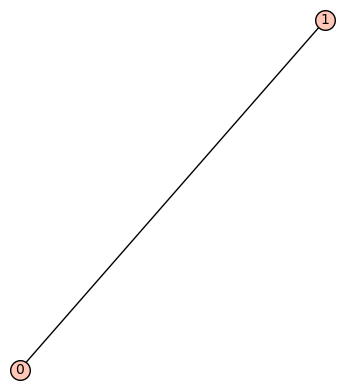
\includegraphics{min_graf_2}
\end{center}

Graf na treh vozliščih. Razlika je $2$.

\begin{center}
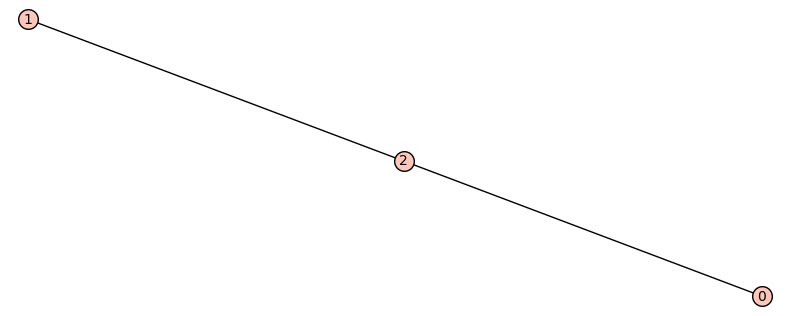
\includegraphics{min_graf_3}
\end{center}

Grafi na štirih vozliščih imajo razliko predpostavke enako $1$.

\begin{center}
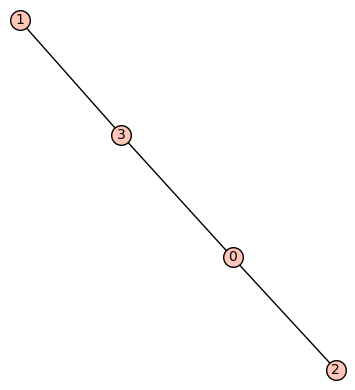
\includegraphics{min_graf_4}
\end{center}

Pri grafih generiranih na petih vozliščih dobiš graf katerega razlika predpostavke je $0$. Generiranih je skupno $21$ grafov na pet vozliščih. Program testira vse te grafe v manj kot $0.2$ sekunde.

\begin{center}
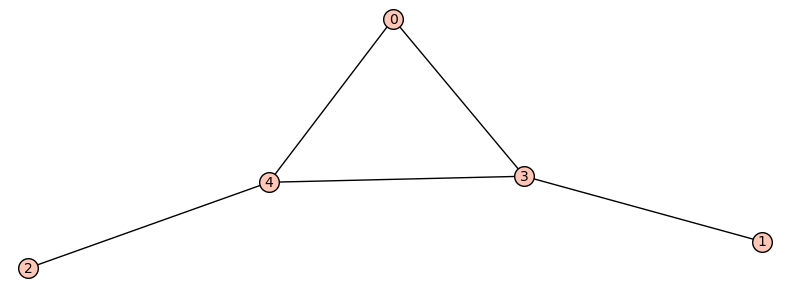
\includegraphics{min_graf_5}
\end{center}

Pri grafih na šest vozliščih je razlika ponovno $0$. Od skupno $112$ vseh možnih grafov na šest vozliščih ima razliko $0$ natanko $8$ grafov. Program testira vse šestvozliščne grafe v približno $0.8$ sekunde. Spodaj je prikazanih pet primerov.

\begin{center}
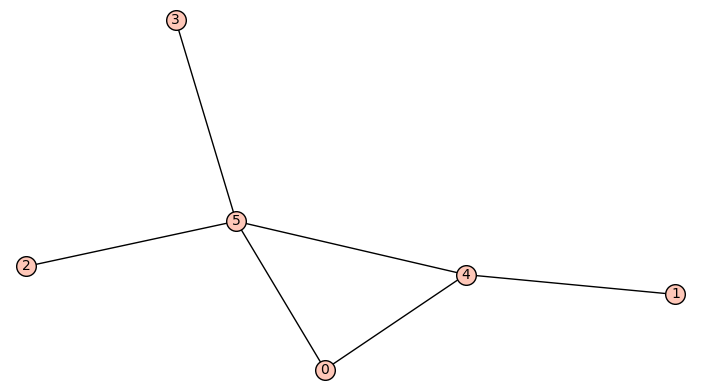
\includegraphics{min_graf_6.1}
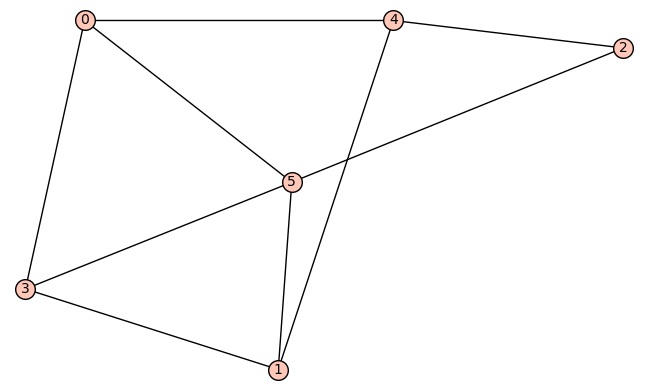
\includegraphics{min_graf_6.2}
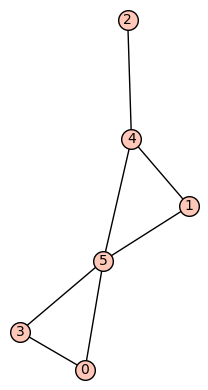
\includegraphics{min_graf_6.3}
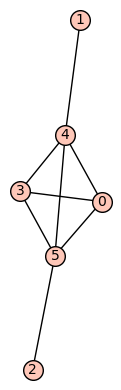
\includegraphics{min_graf_6.4}
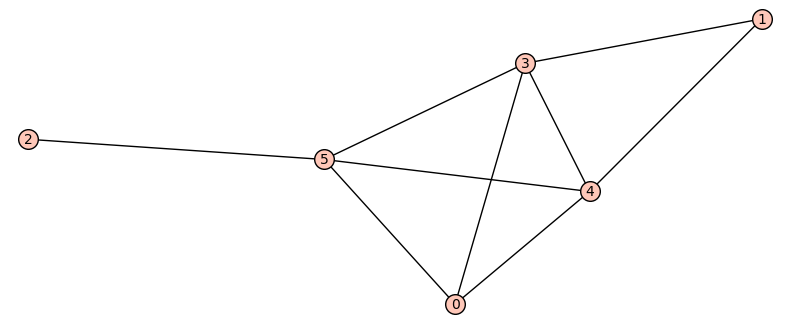
\includegraphics{min_graf_6.5}
\end{center}

Za grafe na sedem vozliščih je minimalna razlika predpostavke ponovno $0$. Sedaj je možno generirati $853$ različnih grafov, razliko $0$ pa jih ima $101$. Program testira to predpostavko na vseh generiranih grafih na sedmih vozliščih v približno $3.7$ sekunde. Ponovno si poglejmo nekaj primerov teh grafov.

\begin{center}
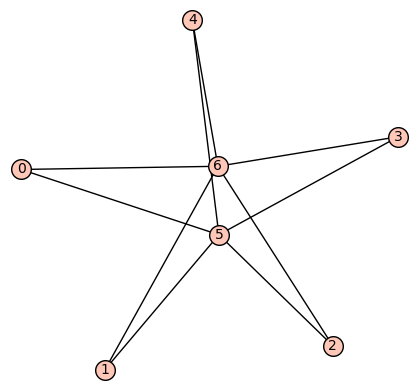
\includegraphics{min_graf_7.1}
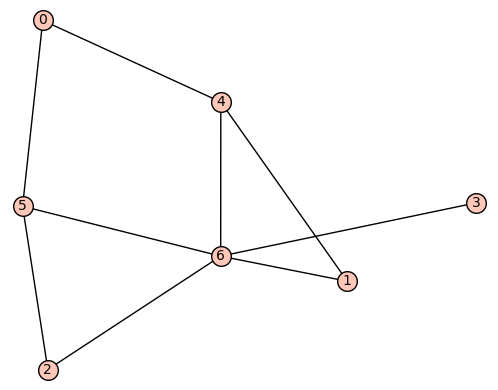
\includegraphics{min_graf_7.2}
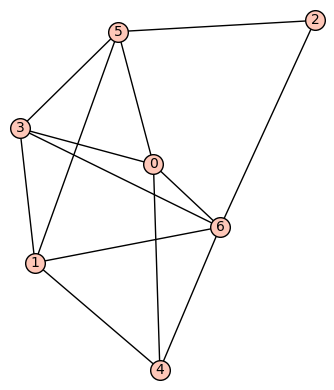
\includegraphics{min_graf_7.3}
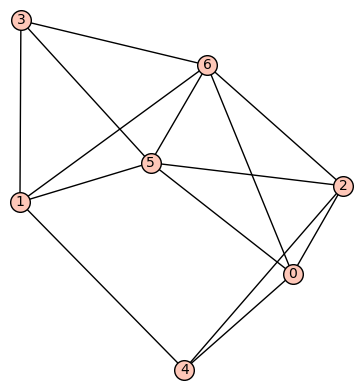
\includegraphics{min_graf_7.4}
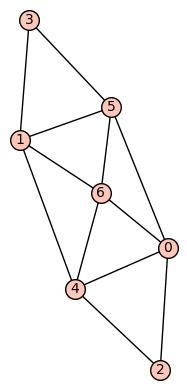
\includegraphics{min_graf_7.5}
\end{center}

Grafi na osmih vozliščih imajo razliko leve in desne strani ponovno enako $0$. Zdaj generiramo že $11117$ različnih grafov in za njihovo testiranje porabimo že kar približno $40$ sekund. Grafov z osmimi vozlišči, kjer je razlika predpostavke enaka $0$ je $1662$.

\begin{center}
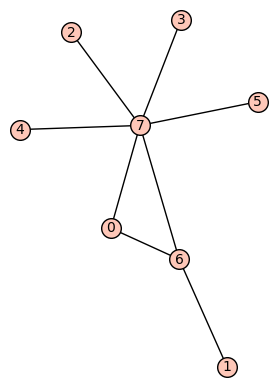
\includegraphics{min_graf_8.1}
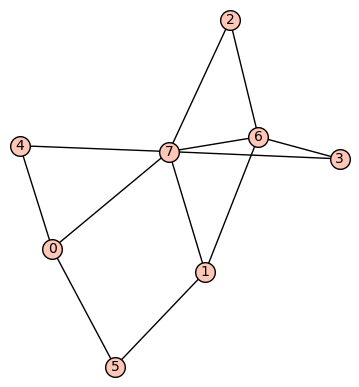
\includegraphics{min_graf_8.2}
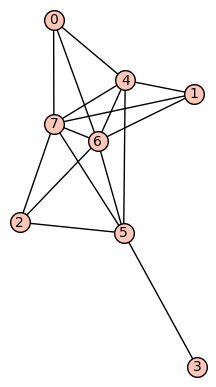
\includegraphics{min_graf_8.3}
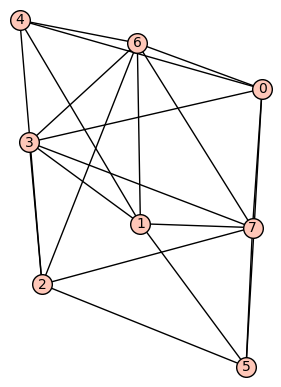
\includegraphics{min_graf_8.4}
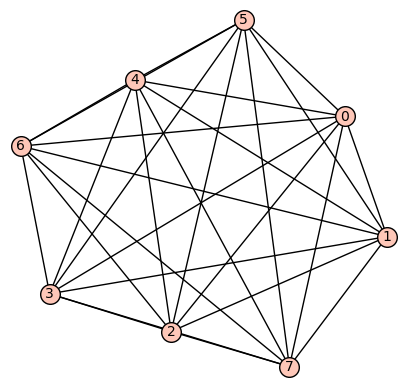
\includegraphics{min_graf_8.5}
\end{center}

Z grafi na osmih vozliščih se konča naše preizkušanje majhnih grafov. Na tej točki računalnik ni več sposoben generirati vseh preprostih povezanih grafov na devetih vozliščih preko generatorja  $graphs.nauty\_geng('v\ -c')$. Portal $CoCalc$ sam terminira generator, če je ta zagnan.

Zaključimo lahko, da dana predpostavka $Graffiti\ conjecture\ 232$ vsekakor velja na majhnih grafih z osem ali manj vozlišči.

\end{document}